\lesson{8}{13.11.2023}{Прямые в пространстве. Эллипс.}


\begin{definition}[Уравнение прямой через 2 точки]
    Пусть есть точки $A(x_1, y_1, z_1)$ и $B(x_2, y_2, z_2)$, тогда уравнение прямой, проходящей через эти точки имеет вид:
    \[\frac{x-x_0}{x_2-x_1} = \frac{y-y_0}{y_2-y_1} = \frac{z-z_0}{z_2-z_1}\]
    т.к. $(x_2-x_1, y_2-y_1, z_2-z_1)$ -- направляющий вектор.
\end{definition}


\section{Угол между прямыми}

\begin{definition}[Угол между прямыми в пространстве]
    \begin{gather*}
        l_1: \frac{x-x_0}{v_1} = \frac{y-y_0}{v_2} = \frac{z-z_0}{v_3}\\
        l_2: \frac{x-x_1}{w_1} = \frac{y-y_1}{w_2} = \frac{z-z_1}{w_3}\\
        \cos\angle(l_1, l_2) = \frac{v_1 w_1 + v_2 w_2 + v_3 w_3}
        {\sqrt{v_1^2+v_2^2+v_3^2} \sqrt{w_1^2+w_2^2+w_3^2}}\\
        l_1 \perp l_2: v_1 w_1 + v_2 w_2 + v_3 w_3  = 0\\
        l_1 \parallel l_2: \frac{v_1}{w_1} = \frac{v_2}{w_2} = \frac{v_3}{w_3}
    \end{gather*}
\end{definition}

Угол между прямой и плоскостью: \\
\noindent\begin{minipage}{0.45\textwidth}
    \begin{gather*}
        l_1: \frac{x-x_0}{v_1} = \frac{y-y_0}{v_2} = \frac{z-z_0}{v_3}\\
        \alpha: Ax+By+Cz+D=0\\
    \end{gather*}
\end{minipage}
\begin{minipage}{0.45\textwidth}
    \begin{center}
        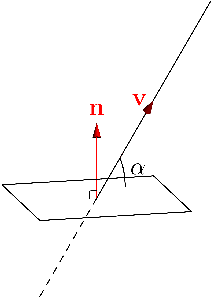
\includegraphics{angle_between_line_and_plane.pdf}
    \end{center}
\end{minipage}
\begin{gather*}
    \sin\theta = \cos \angle (\vn, \vv) = \frac{Av_1 + Bv_2 + Cv_3}
    {\sqrt{A^2+B^2+C^2} \sqrt{v_1^2+v_2^2+v_3^2}}\\
    \alpha \parallel l_1: Av_1 + Bv_2 + Cv_3 = 0\\
    \alpha \perp l_1: \frac{A}{v_1} = \frac{B}{v_2} = \frac{C}{v_3}
\end{gather*}

\begin{theorem}

    $l_1, l_2$ -- пересекаются в одной точке или параллельны
    \[\Leftrightarrow
        \begin{vmatrix}
            x_1 - x_0 & y_1-y_0 & z_1-z_0 \\
            v_1       & v_2     & v_3     \\
            w_1       & w_2     & w_3
        \end{vmatrix} = 0\]
\end{theorem}
\begin{proof}
    $l_1$ и $l_2$ -- в одной плоскости, только если $\vv, \vw$ и
    $(x_1-x_0, y_1-y_0, z_1-z_0)$ в одной плоскости, это равносильно тому, что
    их смешанное произведение равно 0.
\end{proof}

\chapter{Кривые второго порядка}

\section{Эллипс}

\begin{definition}[Стандартный вид прямой II порядка]
    \[a_{11}x^2 + 2a_{12}xy + a_{22}y^2 + b_1x +b_2y +b_3=0\]
    \[a_{11}^2 + a_{12}^2 + a_{22}^2 \neq 0\]
\end{definition}
\begin{definition}\label{def:ellipse1}
    Эллипс --- кривая, которая в подходящих координатах задается уравнением:
    \[\frac{x^2}{a^2} + \frac{y^2}{b^2}=1\]
\end{definition}
\begin{definition}\label{def:ellipse2}
    Пусть $F_1, F_2$ -- точки (фокусы), если $F_1 F_2 = 2c < 2a$, тогда
    ГМТ $M:$ \[F_1M + F_2M=2a\] называется эллипсом.
\end{definition}
\begin{definition}\label{def:ellipse3}
    $F_1$ -- фокус, $l_1$ --  прямая (директриса). ГМТ $M$:
    \[\frac{\dist(F_1,M)}{\dist(l_1,M)} = e < 1\]
    называется эллипсом.
\end{definition}
\begin{minipage}{0.45\textwidth}
    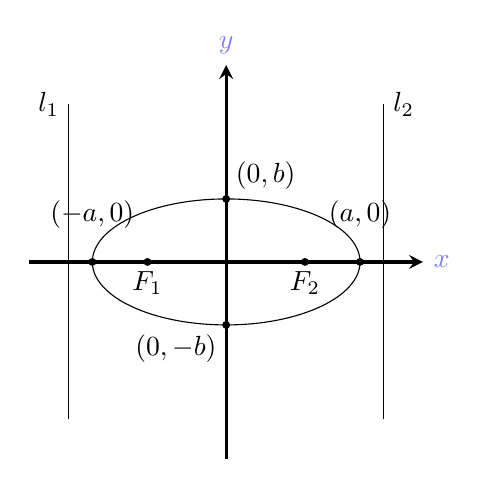
\begin{tikzpicture}
        \tikzset{axis/.style={very thick, ->, >=stealth}}
        \draw[axis] (-2.5, 0) -- (2.5, 0) node [right, color=blue!50] {$x$};
        \draw[axis] (0, -2.5) -- (0, 2.5) node [above, color=blue!50] {$y$};
        \draw (0, 0) ellipse [x radius = 1.7, y radius = 0.8];
        \draw (-1,0) node [below] {$F_1$};
        \fill [black] (-1,0) circle (0.05);
        \draw (1, 0) node [below] {$F_2$};
        \fill [black] (1,0) circle (0.05);
        \draw (-2, -2) -- (-2, 2) node [left] {$l_1$};
        \draw (2, -2) -- (2, 2) node [right] {$l_2$};
        \fill [black] (1.7, 0) circle (0.05);
        \draw (1.7, 0.3) node [anchor=south] {$(a,0)$};
        \fill [black] (-1.7, 0) circle (0.05);
        \draw (-1.7, 0.3) node [anchor=south] {$(-a,0)$};
        \fill [black] (0, 0.8) circle (0.05);
        \draw (0, 0.8) node [anchor=south west] {$(0,b)$};
        \fill [black] (0, -0.8) circle (0.05);
        \draw (0, -0.8) node [anchor=north east] {$(0,-b)$};
    \end{tikzpicture}
\end{minipage}
\begin{minipage}{0.45\textwidth}
    \begin{gather*}
        F_2(c,0) \qquad F_1(-c,0)\\
        l_{1,2}: x = \pm \frac{a}{e}\\
    \end{gather*}
\end{minipage}

\begin{itemize}
    \item $a$ -- большая полуось
    \item $b$ -- малая полуось (по умолчанию $a \ge b$)
    \item $c$ -- фокальный параметр \[a^2 = b^2 + c^2\]
    \item $e = \frac{c}{a} \in \left[0, 1\right)$ -- эксцентриситет
\end{itemize}

\section*{Доказательство}
\begin{itemize}
    \item В определении \ref{def:ellipse1} задано $a,b \implies c = \sqrt{a^2 -b^2}, e = \frac{c}{a}$
    \item В определении \ref{def:ellipse2} задано $a,c \implies b = \sqrt{a^2 -c^2}, e = \frac{c}{a}$
    \item В определении \ref{def:ellipse3} задано $d$ расстояние от фокуса до директрисы. Хотим $F(c,0);l:x = \frac{a}{e}$
          \begin{gather*}
              d = \frac{a}{e} -c = \frac{a}{e} - ae = a \left(\frac{1}{e}-e\right)\\
              a = \frac{d}{\frac{1}{e}-e}\\
              c=ae; b = \sqrt{a^2 -c^2}
          \end{gather*}
\end{itemize}

\begin{theorem}
    Определения \ref{def:ellipse1}, \ref{def:ellipse2} и \ref{def:ellipse3} равносильны.
\end{theorem}
\begin{proof}
    Докажем, что \ref{def:ellipse1} и \ref{def:ellipse2} равносильны:

    \noindent\begin{minipage}{0.45\textwidth}
        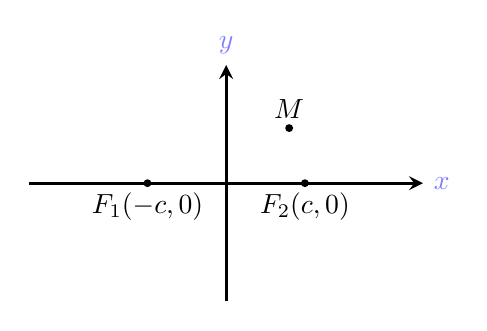
\begin{tikzpicture}
            \tikzset{axis/.style={very thick, ->, >=stealth}}
            \draw[axis] (-2.5, 0) -- (2.5, 0) node [right, color=blue!50] {$x$};
            \draw[axis] (0, -1.5) -- (0, 1.5) node [above, color=blue!50] {$y$};
            \draw (-1,0) node [below] {$F_1 (-c, 0)$};
            \fill [black] (-1,0) circle (0.05);
            \draw (1, 0) node [below] {$F_2 (c,0)$};
            \fill [black] (1,0) circle (0.05);
            \draw (0.8, 0.7) node [above] {$M$};
            \fill [black] (0.8, 0.7) circle (0.05);
        \end{tikzpicture}
    \end{minipage}
    \begin{minipage}{0.45\textwidth}
        \begin{gather*}
            F_1M+F_2M = 2a\\
            F_1M = \sqrt{(x+c)^2 + y^2}\\
            F_2M = \sqrt{(x-c)^2 + y^2}
        \end{gather*}
    \end{minipage}
    \begin{gather*}
        \sqrt{(x+c)^2 + y^2} + \sqrt{(x-c)^2 + y^2} = 2a\\
        \sqrt{(x+c)^2 + y^2} = 2a - \sqrt{(x-c)^2 + y^2}\\
        x^2 + 2cx +c^2 + y^2 = 4a^2 + x^2 - 2cx + c^2 + y^2 - 4a \sqrt{(x-c)^2 + y^2}\\
        4a \sqrt{(x-c)^2 + y^2} = 4a^2 - 4cx\quad |:4a\\
        \intertext{Расстояние от точки на эллипсе до фокуса}
        \boxed{\sqrt{(x-c)^2 + y^2} = a - ex} \qquad \boxed{\sqrt{(x+c)^2 + y^2} = a + ex}\\
        (x-c)^2 + y^2 = a^2 - 2aex +e^2x^2\\
        x^2 -2cx +c^2 +y^2 = a^2 -2aex + e^2x^2\\
        x^2(1-e^2) + y^2 = a^2 -c^2 =b^2\\
        x^2 \frac{1-e^2}{b^2} + \frac{y^2}{b^2} = 1\\
        \intertext{Нужно доказать, что:}
        \frac{b^2}{1-e^2} = a^2\\
        b^2 = a^2 -a^2e^2 \qquad a^2 e^2 = c^2\\
        \frac{x^2}{a^2} + \frac{y^2}{b^2}=1 \qedhere
    \end{gather*}
\end{proof}
\begin{proof}
    Докажем, что \ref{def:ellipse1} и \ref{def:ellipse3} равносильны:

    \noindent\begin{minipage}{0.3\textwidth}
        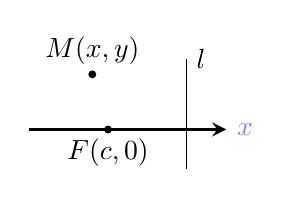
\begin{tikzpicture}
            \tikzset{axis/.style={very thick, ->, >=stealth}}
            \draw[axis] (0, 0) -- (2.5, 0) node [right, color=blue!50] {$x$};
            \draw (1, 0) node [below] {$F(c,0)$};
            \fill [black] (1,0) circle (0.05);
            \draw (0.8, 0.7) node [above] {$M(x,y)$};
            \fill [black] (0.8, 0.7) circle (0.05);
            \draw (2, -0.5) -- (2, 0.9) node [right] {$l$};
        \end{tikzpicture}
    \end{minipage}
    \begin{minipage}{0.60\textwidth}
        \begin{gather*}
            l: x = \frac{a}{e} \qquad \frac{\sqrt{(x-c)^2 + y^2}}{\frac{a}{e}-x} = e\\
            \sqrt{(x-c)^2 + y^2} = e\left(\frac{a}{e}-x\right) = a-ex
        \end{gather*}
    \end{minipage}

    Далее смотри равносильность \ref{def:ellipse1} и \ref{def:ellipse2}.
\end{proof}


\begin{theorem}
    Прямая $Ax + By + C = 0$ касается эллипса $\frac{x^2}{a^2} + \frac{y^2}{b^2} =1$
    \[\Leftrightarrow A^2 a^2 + B^2 b^2 = C^2\]
\end{theorem}
\begin{proof}
    Касательная имеет 1 точку пересечения с эллипсом
    \begin{gather*}
        B \neq 0 \qquad
        y = \frac{-C-Ax}{B} \qquad
        \frac{x^2}{a^2} + \frac{\left(\frac{C+Ax}{B}\right)^2}{b^2} = 1\\
        x^2b^2B^2 + a^2C^2 + a^2A^2x^2 + 2a^2ACx = a^2 b^2 B^2\\
        x^2(a^2A^2 + b^2B^2) + 2a^2ACx + \left(a^2C^2 - a^2b^2B^2\right)=0\\
        \intertext{Это уравнение имеет ровно 1 корень}
        \frac{D}{4} = 0 \qquad
        a^4 A^2 C^2 - (a^2C^2 - a^2 b^2 B^2)(a^2A^2 + b^2B^2)=0\\
        a^2 A^2 C^2 - (C^2 - b^2 B^2)(a^2A^2 + b^2B^2)=0\\
        a^2 A^2 C^2 - a^2 A^2 C^2 - b^2B^2 C^2 + a^2b^2A^2B^2 + b^4B^4=0\\
        a^2b^2A^2B^2 + b^4B^4 = b^2B^2 C^2 \\
        a^2A^2 + b^2B^2 =  C^2
    \end{gather*}
\end{proof}